%% LaTeX2e class for student theses
%% sections/content.tex
%% 
%% Karlsruhe Institute of Technology
%% Institute for Program Structures and Data Organization
%% Chair for Software Design and Quality (SDQ)
%%
%% Dr.-Ing. Erik Burger
%% burger@kit.edu
%%
%% Version 1.3.2, 2017-08-01

\chapter{Design of a TDNN acoustic model}
\label{ch:tdnn_design}
Our approach for creating a robust TDNN acoustic model is to find a TDNN model that performs good on clean data first. Therefore, we had to make several design decisions. Most of the design decisions were justified by experiments, while some were taken from related work. This chapter summarizes the decisions made and the corresponding results. It should be noted that the experiments about robust acoustic modeling with TDNNs described in \cite{peddinti2015jhu} and \cite{peddinti2015reverberation} provided the main motivation for this work, therefore we based some of our parameters on their result.
\section{Training Data and System Setup}
All experiments in this work only concern the neural network part of our acoustic model, which is a HMM/TDNN hybrid. The speech recognition system itself, as well as all data, the HMM part of the acoustic model, the dictionary and the language model, are based upon the system described in \cite{nguyen20162016}. The system is built upon the Janus recognition toolkit \cite{finke1997karlsruhe}. We utilize a four-gram language model and the CMU Pronouncing Dictionary \cite{cmudict}, which uses 39 phones. The acoustic model uses quinphones and has 8156 different distributions, which means that the HMM part of our acoustic model has 8156 different states. \\ \\
The training and test dataset for the acoustic model consist of 468 hours of English speech from the TED-LIUM v2 \cite{rousseau2014enhancing}, Broadcast News \cite{graff19971996} and Quaero 2010-2012 datasets. From these 468~hours, 17~hours are randomly selected as test set, 451~hours are used for the training set. \\ \\
The development dataset, used for tuning the decoder parameters, consists of the english IWSLT 2013 evaluation dataset for the ASR track \cite{cettolo2013report}. This dataset consists of 3.9~hours of TED talks. The word error rates for all experiments in this chapter were measured on this development set. \\ \\ 
Each frame of samples in the datasets consists of 40~log-mel features which were normalized over the whole utterance to have mean zero and variance two. Each frame covers 32~milliseconds. The frame shift between successive frames is 10~milliseconds. The sampling rate of the audio data was 16~kHz. \\ \\
The neural network training was done using a custom framework, build on top of PyTorch \cite{paszke2017automatic}. Pytorch is a machine learning framework that supports GPU accelleration, parallelization along multiple systems and automatic differentiation. In the context of this work, several contributions were made to the PyTorch framework.  
\section{Neural Network Parameters}
This section focuses on parameters that are related to the neural network design. For all models in this section, the word error rate was estimated by using $l_p$ and $l_z$ that were tuned for each model separately. The priors were estimated by counting labels over the whole training set.
\subsection{Input Context}
The time input context of all our TDNN models is $(-13,9)$, which means the TDNN sees the current frame, thirteen frames in the past, and nine frames in the future. This parameter was taken from the smallest TDNN model described in \cite{peddinti2015reverberation}.
\subsection{Count and Width of Layers}
The count of layers and width of each layer is one of the most important design parameters for neural networks. As in \cite{peddinti2015reverberation}, all our models use the same amount of channels for each TDNN layer. Only the count of observed time frames changes with each layer. \\ \\
\begin{minipage}{\linewidth}
	\centering
	\begin{tabular}{@{\extracolsep{4pt}}lccccccccc@{}}
		\toprule
		Model:      & \multicolumn{4}{c}{Four Layer}       & \multicolumn{5}{c}{Five Layer}\\\cmidrule[1pt]{1-1}\cmidrule[1pt]{2-5}\cmidrule[1pt]{6-10}
		Layer       & 1 & 2 & 3 & 4    & 1 & 2 & 3 & 4 & 5 \\\cmidrule{2-5}\cmidrule{6-10}
		Kernel Size & 5 & 2 & 2 & 2    & 5 & 5 & 3 & 2 & 2 \\
		Stride      & 3 & 2 & 2 & 2    & 2 & 1 & 1 & 1 & 1 \\
		\bottomrule
	\end{tabular}
	\captionof{table}{Kernel size and stride parameters for the two different architectures}
	\label{tbl:tdnn_layer_design}
\end{minipage} \\ \\
We decided to test a four layer model with exactly the same parameters as the smallest model in \cite{peddinti2015reverberation}. This model also included a splicing layer after layer one. The splicing configuration was $(0, 1, 2, 3, 3, 4, 5, 6)$, relative to the previous layer. For the second model we tested, we decided to use larger kernels and one more layer. For this purpose, we removed the splicing layer and increased the layer count to five. Table \ref{tbl:tdnn_layer_design} gives the kernel size and stride over time for each layer in each architecture. For both models, we used an L2 pooling nonlinearity with group size of ten followed by a batch normalization layer after each TDNN layer.
\\
Figure \ref{fig:tdnn_layer_design} shows the word error rate for the two different architectures, given the count of channels. It can be seen that the four-layer architecture performed better than the five-layer architecture. We found the optimal count of channels  for the four-layer model to be 300. This contradicts \cite{peddinti2015reverberation}, where 400 channels were used. \\ \\
\begin{minipage}{\linewidth}
	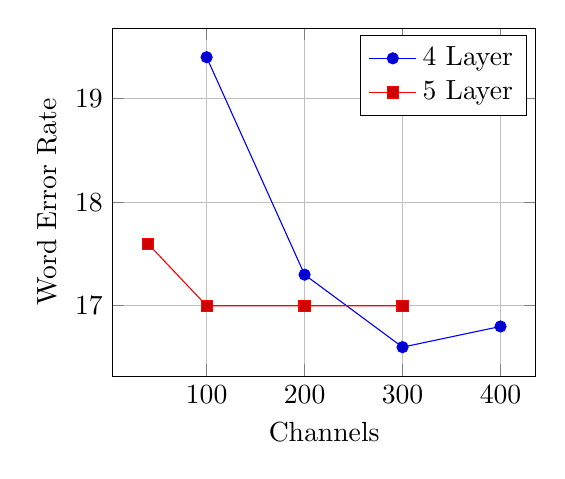
\begin{tikzpicture}
	\begin{axis}[ylabel=Word Error Rate, xlabel=Channels, height=6cm, 
	xticklabel style={name=T\ticknum},grid=major]
	\addplot coordinates {
		(100,19.4) %994
		(200,17.3) %999
		(300,16.6) %1009
		(400,16.8) %1010
	};
	\addlegendentry{4 Layer};
	\addplot coordinates {
		(40,17.6) %1040
		(100,17.0) %i3
		(200,17.0) %1039
		(300,17.0) %1036
	};
	\addlegendentry{5 Layer};
	\end{axis}
	\end{tikzpicture}
	\captionof{figure}{Word Error Rate for different choices of layer and channel count}
	\label{fig:tdnn_layer_design}
\end{minipage} 
\subsection{Nonlinearity}
\label{sec:tdnn_nonlin}
Following \cite{zhang2014improving}, we tested L2 pooling nonlinearity with group size if ten after each TDNN layer. Using the L2 norm can be problematic, as the gradient is not defined when all inputs in the pooling group are zero. The authors of \cite{zhang2014improving} propose to use a modified batch normalization layer after each LP-pooling layer, which solves the problem. We propose an alternate approach, which is setting the gradient to zero if all inputs become zero. Furthermore, we also tested max pooling as a possible nonlinearity. All experiments were conducted on the four-layer architecture described before. Figure \ref{fig:tdnn_nonlinearity} shows the results. \\ \\
\begin{minipage}{\linewidth}
	\centering
	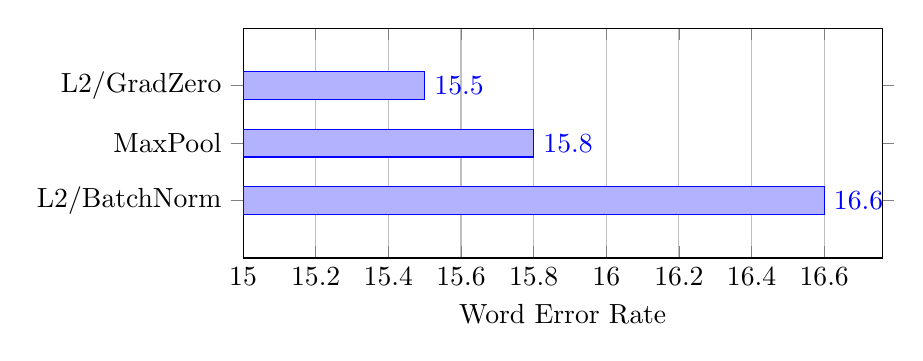
\begin{tikzpicture}
		\begin{axis}[
		xbar,xmajorgrids=true,
		width=0.8\linewidth,height=4.5cm, enlarge y limits=0.5,
		xmin=15,xlabel={Word Error Rate},
		symbolic y coords={L2/BatchNorm,MaxPool,L2/GradZero},
		ytick=data,nodes near coords, nodes near coords align={horizontal},
		]
		%1009, I24, I12
		% All with only l[/lz/mb tuning, no custom priors and no softmax
		\addplot coordinates {(15.5,L2/GradZero) (15.8,MaxPool) 
		(16.6,L2/BatchNorm)};
		\end{axis}
	\end{tikzpicture}
	\captionof{figure}{Word Error Rate for different choices of nonlinearities}
	\label{fig:tdnn_nonlinearity}
\end{minipage} \\ \\
In our case, the usage of L2 pooling with a modified gradient outperformed the other nonlinearities. It was not possible to compare L2 pooling without any modifications, as our training became unstable. 
\section{Training Setup}
This section is focused on the training setup for our acoustic model. Out setup is closely related to the setup described in \cite{nguyen20162016}. We essentially use the same speech recognition system, the same labels, as well as the same samples for training our acoustic model.
\subsection{Shuffling and Preparation of Dataset}
For our experiments, we benchmarked different shuffling strategies with a six-layer fully connected network. Shuffling of the whole dataset once before training, and shuffling of the whole dataset before each epoch. The results can be seen in figure \ref{fig:tdnn_shuffling}. \\ \\
\begin{minipage}{\linewidth}
	\centering
	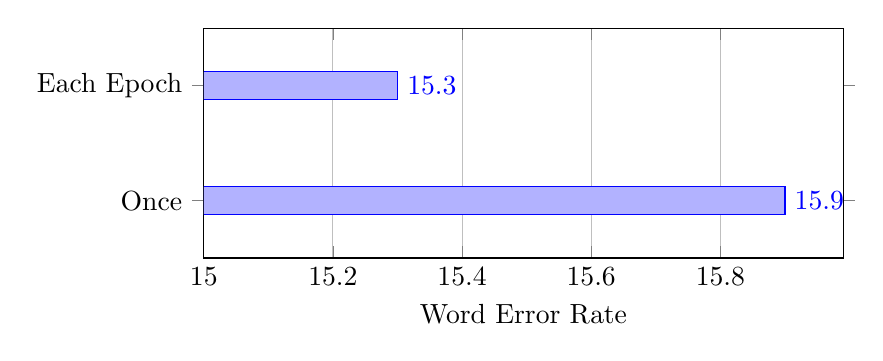
\begin{tikzpicture}
	\begin{axis}[
	xbar,xmajorgrids=true,
	width=0.8\linewidth,height=4.5cm, enlarge y limits=0.5,
	xmin=15,xlabel={Word Error Rate},
	symbolic y coords={Once,Each Epoch},
	ytick=data,nodes near coords, nodes near coords align={horizontal},
	]
	\addplot coordinates {(15.9,Once) (15.3,Each Epoch)};
	\end{axis}
	\end{tikzpicture}
	\captionof{figure}{Word Error Rate for different shuffling strategies}
	\label{fig:tdnn_shuffling}
\end{minipage} \\ \\
We can see that shuffling of the training dataset before each epoch decreased the word error rate. \\
\subsection{Learning Rate and Learning Rate Decay}
As in \cite{nguyen20162016}, we utilize the newbob learning rate scheduler for training for stochastic gradient descend, with an initial learning rate of $0.08$ and a momentum of $5$. The SGD variant used is the introduced in section \ref{sec:momentum}, as this was also used in \cite{nguyen20162016}\footnote{This SGD variant is not equal to the default SGD variant implemented in pytorch.}. Figure \ref{fig:newbob_wer} shows the word error rate per epoch when using newbob. It can be seen that there were almost no improvements during epoch four, but the word error rate improved as soon as the decaying started after epoch four. Figure \ref{fig:newbob_fer} shows the frame error rate per epoch for the same training run. It can be seen that exponential decay reduces the frame error rate significantly. The model used for this experiment was the four layer TDNN introduced in the previous section.
\\ \\
\begin{minipage}{\linewidth}
	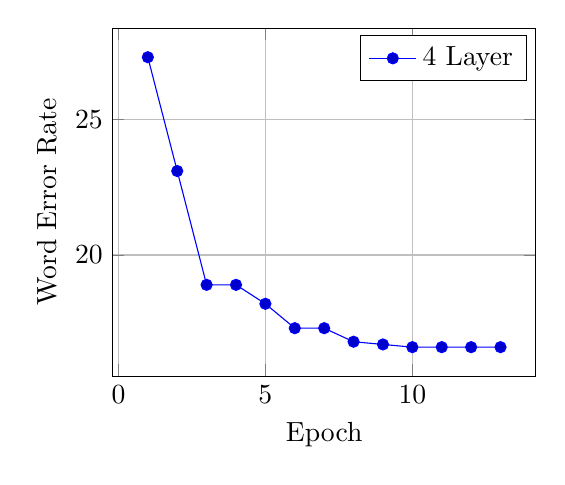
\begin{tikzpicture}
	\begin{axis}[ylabel=Word Error Rate, xlabel=Epoch, height=6cm, 
	xticklabel style={name=T\ticknum},grid=major]
	% I12
	\addplot coordinates {
		(1,27.3)
		(2,23.1)
		(3,18.9)
		(4,18.9)
		(5,18.2)
		(6,17.3)
		(7,17.3)
		(8,16.8)		
		(9,16.7)
		(10,16.6)
		(11,16.6)
		(12,16.6)
		(13,16.6)
	};
	\addlegendentry{4 Layer};
	\end{axis}
	\end{tikzpicture}
	\captionof{figure}{Word Error Rate per Epoch when using newbob training. The exponential decaying of the learning rate started after epoch four.}
	\label{fig:newbob_wer}
\end{minipage}
 \\ \\
\begin{minipage}{\linewidth}
	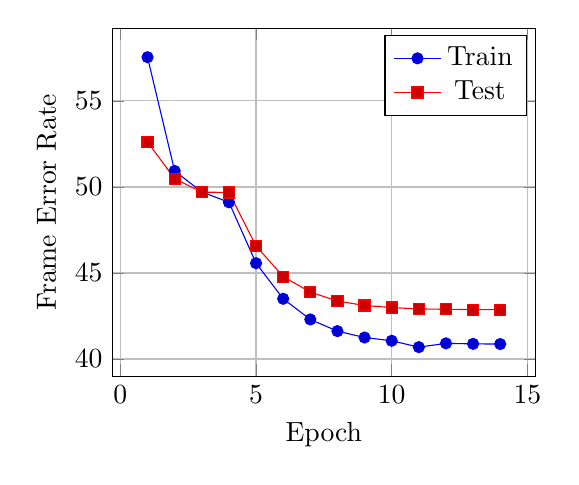
\begin{tikzpicture}
	\begin{axis}[ylabel=Frame Error Rate, xlabel=Epoch, height=6cm, 
	xticklabel style={name=T\ticknum},grid=major]
	%I12
	\addplot coordinates {
		(1,57.54)
		(2,50.93)
		(3,49.71)
		(4,49.11)
		(5,45.57)
		(6,43.50)
		(7,42.30)
		(8,41.62)		
		(9,41.25)
		(10,41.06)
		(11,40.69)
		(12,40.91)
		(13,40.88)
		(14,40.87)
	};
	\addlegendentry{Train};
	\addplot coordinates {
		(1,52.61)
		(2,50.48)
		(3,49.70)
		(4,49.68)
		(5,46.57)
		(6,44.79)
		(7,43.89)
		(8,43.37)		
		(9,43.11)
		(10,42.99)
		(11,42.91)
		(12,42.89)
		(13,42.87)
		(14,42.87)
	};
	\addlegendentry{Test};
	\end{axis}
	\end{tikzpicture}
	\captionof{figure}{Frame Error Rate per Epoch when using newbob training. The exponential decaying of the learning rate started after epoch four.}
	\label{fig:newbob_fer}
\end{minipage}
\subsection{MMIE Training}
Since the experiments described in \cite{peddinti2015jhu} show improvement when sMBR discriminative training is used, we attempted to use discriminative based training as well. Our implementation used maximum mutual information estimation, as described in section \ref{sec:mmie}. We picked this training variant as a first step, since it is easier to implement than any variant of overall risk criterion estimation. Both approaches should show some improvement over cross entropy loss on frame level, according to several bodies of work \cite{povey2005discriminative} \cite{ghoshal2013sequence}. \\ \\
For MMIE training, we pre-trained a four layer TDNN acoustic model with frame-based cross entropy loss for a single epoch. Then, we started MMIE training on a per-utterance basis. For this purpose, we wrote a module that enabled interoperability between the Janus recognition toolkit and PyTorch. The training was done on multiple machines with a total of 256 processors, the gradients were averaged before each SGD step. \\ \\
While our experiments consistently showed high improvements in terms of frame error rate, the word error rate increased significantly: The model reached a WER of $17.6$ using cross entropy loss, but only a WER $25.6$ was reached after the MMIE training finished the first epoch. This effect was also described in more practically oriented literature \cite{su2013error} for MMIE without any further modifications. 

\begin{minipage}{\linewidth}
	\begin{minipage}{0.5\linewidth}
	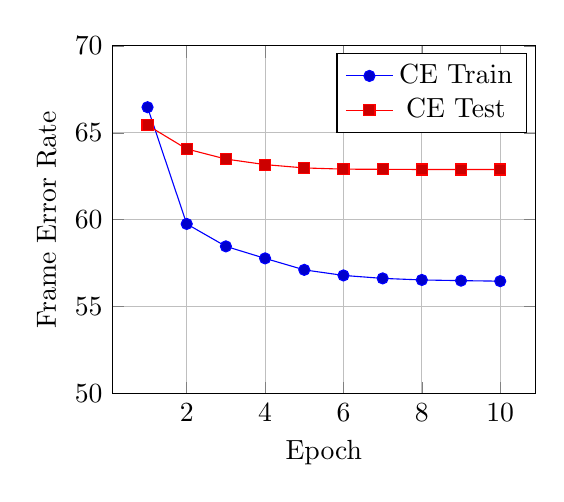
\begin{tikzpicture}
	\begin{axis}[ylabel=Frame Error Rate, xlabel=Epoch, height=6cm, 
	ymin=50, ymax=70,
	xticklabel style={name=T\ticknum},grid=major]
	%1040
	\addplot coordinates {
		(1,66.47)
		(2,59.76)
		(3,58.47)
		(4,57.78)
		(5,57.12)
		(6,56.80)
		(7,56.63)
		(8,56.54)		
		(9,56.50)
		(10,56.47)
	};
	\addlegendentry{CE Train};
	\addplot coordinates {
		(1,65.43)
		(2,64.07)
		(3,63.49)
		(4,63.17)
		(5,62.98)
		(6,62.91)
		(7,62.90)
		(8,62.89)		
		(9,62.89)
		(10,62.89)
	};
	\addlegendentry{CE Test};
	\end{axis}
	\end{tikzpicture}
\end{minipage}
\hfill
\begin{minipage}{0.5\linewidth}
	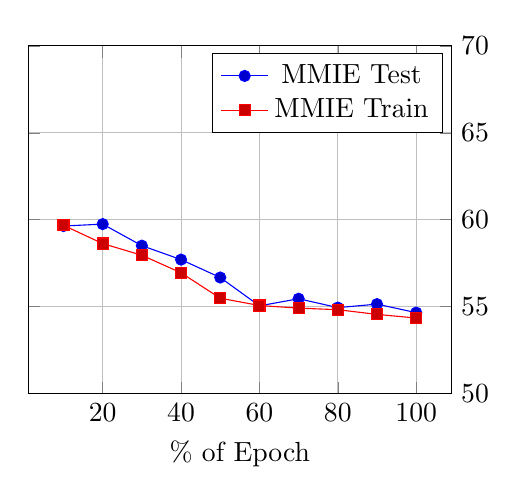
\begin{tikzpicture}
	\begin{axis}[xlabel=\% of Epoch, height=6cm, 
	 ylabel near ticks, yticklabel pos=right,
	ymin=50, ymax=70,
	xticklabel style={name=T\ticknum},grid=major]
	%1040 SMBR 24
	\addplot coordinates {
		(10,59.64)
		(20,59.75)
		(30,58.51)
		(40,57.71)
		(50,56.68)
		(60,55.05)
		(70,55.46)
		(80,54.95)		
		(90,55.15)
		(100,54.66)
	};
	\addlegendentry{MMIE Test};
	\addplot coordinates {
		(10,59.68)
		(20,58.631)
		(30,57.96)
		(40,56.95)
		(50,55.49)
		(60,55.07)
		(70,54.92)
		(80,54.83)		
		(90,54.56)
		(100,54.35)
	};
	\addlegendentry{MMIE Train};
	\end{axis}
	\end{tikzpicture}
\end{minipage}
	\captionof{figure}{Frame Error Rate per Epoch when using cross entropy loss, as well as Frame Error Rate over a single epoch when using MMIE on a TDNN}
	\label{fig:mmie_fer}
\end{minipage} \\ \\
Detailed results regarding the frame error rate are shown in figure \ref{fig:mmie_fer}. It can be seen that the MMIE training converged significantly faster than cross entropy training. Also, the error on the test data set is significantly closer to the error on the training data set. 
\iffalse
% This is the training for a Fully Connected net with ReLU, which diverged. There are examples in the litherature which did NOT diverge. 
\begin{minipage}{\linewidth}
	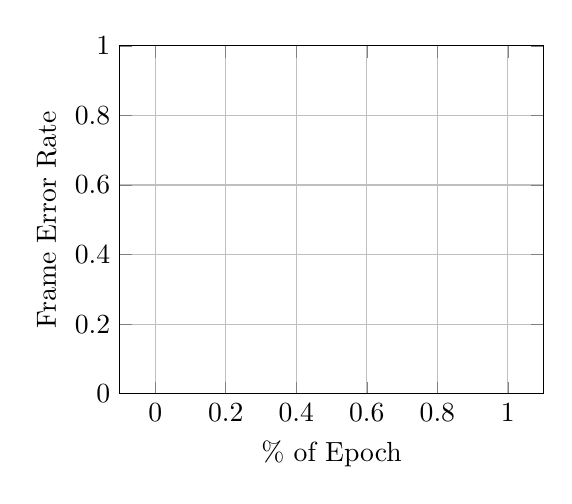
\begin{tikzpicture}
	\begin{axis}[ylabel=Frame Error Rate, xlabel=\% of Epoch, height=6cm, 
	ymin=50, ymax=70,
	xticklabel style={name=T\ticknum},grid=major]
	%1040
	\addplot coordinates {
		(10,75.2618)
		(20,75.2638)
		(30,75.2839)
		(40,76.25)
		(50,76.99539216)
		(60,87.03598039)
		(70,83.21137255)
		(80, 84.23852941)
	};
	\addlegendentry{MMIE Train};
	\end{axis}
	\end{tikzpicture}
	\label{fig:mmie_fer_fc}
\end{minipage}
\fi
\\ These results were achieved using the four-layer TDNN model. Caution has to be taken when interpreting the results: While the amount of data in both test data sets is the same, they are not equal as training and testing for MMIE happens on per-utterance basis, while the test and training sets for the cross entropy loss based training were created on per-frame basis. \\ \\
Although the results regarding frame error rate look interesting, we did not pursue this approach any further, due to the resulting high word-error rates and the numerous details one has to consider for working MMIE training on neural networks \cite{su2013error}.

\section{Decoding Parameters}
Tuning decoding parameters is important for good achieving a high accuracy on word level. The decoding parameters are not directly related to the acoustic model, but rather the decoding process. Different acoustic models might still require different decoding parameters for best performance. 
\subsection{Acoustic Model Scaling and Length Penalty}
Our experiments have shown that the $l_p$ and $l_z$ parameters are depending on each other. Therefore we can not optimize them separately. We choose to perform a grid search over a reasonable parameter space. \\ \\
\begin{minipage}{\linewidth}
\centering
\begin{tikzpicture}
\begin{axis}[grid=both,zlabel=Word Error Rate,xlabel=$l_p$,ylabel=$l_z$,width=0.7\linewidth]
	\addplot3[surf,mesh/cols=10,z buffer=sort] file {data/lp_lz_i12};
\end{axis}
\end{tikzpicture}
\captionof{figure}{Illustrative example of the word error rate for different $l_p$ and $l_z$ parameters for a four-layer TDNN}
\label{fig:lp_lz}
\end{minipage}
\\ \\
An example impact of the $l_p$ and $l_z$ for two different models are illustrated in figure \ref{fig:lp_lz}. Our experiments have shown that the optimal parameters are similar for each of the models we tested. It is still advisable to fine tune the parameters for each model. Taking the initial values for the grid search from an similar model usually leads to good results.
\subsection{Master Beam}
We tested several architectures with different master beams. Master beams between four and six appeared to work best, but we did not find any pattern that correlated with the network architecture. This indicates that the optimal master beam depends on several factors, not just on the architecture of the neural network model itself. 
\subsection{Neural Network Priors}
\label{sec:tdnn_prior}
As described in section \ref{sec:ce_loss}, it is important to scale the posteriors generated by the neural network with priors. We tested two different approaches of generating the priors: Generating them from the complete test dataset and also generating them from the output of a trained model. In the second case, we selected thirty minutes of speech data randomly from our dataset, computed the neural network output on it, and counted the occurrence of each label in the output. \\ \\
\begin{minipage}{\linewidth}
	\centering
	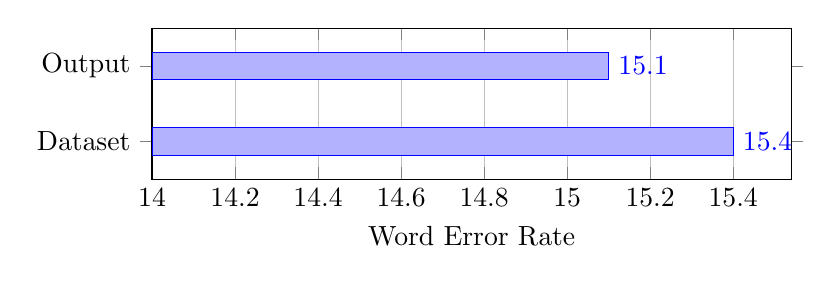
\begin{tikzpicture}
	\begin{axis}[
	xbar,xmajorgrids=true,
	width=0.8\linewidth,height=3.5cm, enlarge y limits=0.5,
	xmin=14,xlabel={Word Error Rate},
	symbolic y coords={Dataset,Output},
	ytick=data,nodes near coords, nodes near coords align={horizontal},
	]
	\addplot coordinates {(15.4,Dataset) (15.1,Output)};
	\end{axis}
	\end{tikzpicture}
	\captionof{figure}{Word Error Rate for priors estimated from the dataset and the model output}
	\label{fig:wer_priors}
\end{minipage} 
\\
As illustrated in figure \ref{fig:wer_priors}, calculating the priors from the output of the model decreased the word error rate significantly. These experiments were done on the four-layered TDNN model. 
\subsection{Softmax Smoothing}
We also tested the impact of softmax smoothing on the neural network output. The motivation is that a beam search through a hidden Markov model does not work very well when the acoustic model is overconfident regarding certain states. Figure \ref{fig:softmax_fer} shows that softmax smoothing decreased the word error rate for our four-layer TDNN model. \\ \\
\begin{minipage}{\linewidth}
	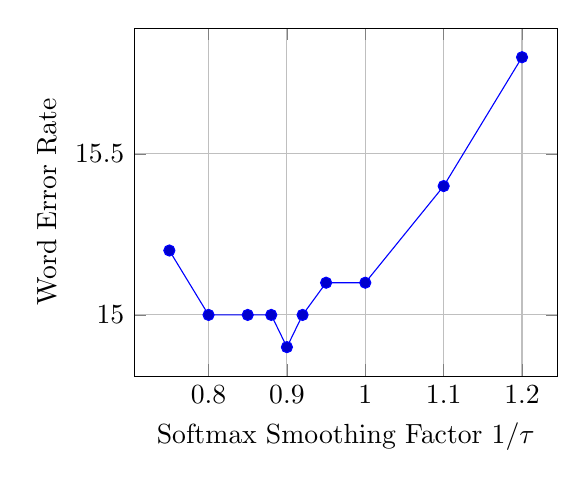
\begin{tikzpicture}
	\begin{axis}[ylabel=Word Error Rate, xlabel=Softmax Smoothing Factor $1/\tau$, height=6cm, 
	xticklabel style={name=T\ticknum},grid=major]
	%I12
	\addplot coordinates {
		(0.75,15.2)
		(0.8,15)
		(0.85,15)
		(0.88,15)
		(0.9,14.9)
		(0.92,15)
		(0.95,15.1)
		(1,15.1)
		(1.1,15.4)
		(1.2,15.8)
	};
	\end{axis}
	\end{tikzpicture}
	\captionof{figure}{Word Error Rate per softmax adjustment $1/\tau$ for a four-layer TDNN model}
	\label{fig:softmax_fer}
\end{minipage} \\ \\


\iffalse
\label{ch:approach}
This chapter describes our approach for acoustic modelling using TDNNs on a high level. 
We will also give a brief overview over unknown hyperparemters and design decisions,
as well as a coarse overview over the structure of our implementation. 

\chapter{Experiment Setup}
\label{ch:experiment_setup}
This chapter should describe the detailed preleminaries and hyperparemters of our training and evaluation setup:
\begin{itemize}
    \item which data, and which preprocessing was used
    \item how was the data reverbed
    \item which learning rate schedulers, optimizers, loss functions were used
    \item which mechanisms were used to make the training faster and scalable
\end{itemize}
\fi